\subsection{Software Architecture}
Although not strictly part of the hardware system, the software architecture is what connects, manages, and coordinates all onboard components. It defines how the sensors, actuators, and computational units communicate to form a complete autonomous system. The design follows a modular and distributed approach, separating computational loads across multiple processors to improve reliability, maintainability, and scalability. This structure also allows new hardware, such as the side scan sonar, to be integrated seamlessly without major reconfiguration of existing modules.
\\ \\
Each subsystem is assigned a specific computational domain with a well-defined purpose. The \textit{``Navigation Unit''} on the \textit{``LattePanda 3 Delta''} is responsible for low-level control, sensor fusion, and actuator management, interfacing directly with the IMU, GNSS, and thruster controllers. The \textit{``Perception Unit''} on the \textit{``NVIDIA Jetson Orin NX''} handles high bandwidth sensors such as LiDAR and stereo cameras, performing real-time perception, object detection, and mapping. The \textit{``Ground Control Station''} provides remote supervision, telemetry visualization, and manual override when required. Together, these systems operate in a synchronized local Ethernet network, exchanging data through a standardized message layer.
\\ \\
The software stack runs on \textit{``Ubuntu 24.04 LTS''} with the \textit{``ROS2 Jazzy Jalisco''} distribution. ROS2 acts as the communication backbone, providing a real-time publish/subscribe framework through the Data Distribution Service (DDS) middleware. Each functional block in the system is implemented as an independent ROS2 node that communicates via topics, services, and actions. This decoupled design simplifies debugging, system upgrades, and integration of experimental modules for research.
\\ \\
A key part of the architecture is precise time synchronization between all onboard computers. The system uses a hardware signal called Pulse Per Second (PPS) from the GNSS modules to align the internal clocks of each computer. This signal marks the exact start of every second and is combined with the GNSS time data to keep all systems synchronized. A background process running in Linux automatically adjusts the system clocks based on this information, ensuring that all sensor data are timestamped with the same reference time. This sub-microsecond synchronization is essential for accurate sensor fusion, navigation, and SLAM.
\\ \\
An overview of the complete software architecture and node interconnections is shown in Figure~\ref{fig:microAmpere-software-architecture-overview} down below on the next page.

\newpage

\begin{figure}[H]
    \centering
    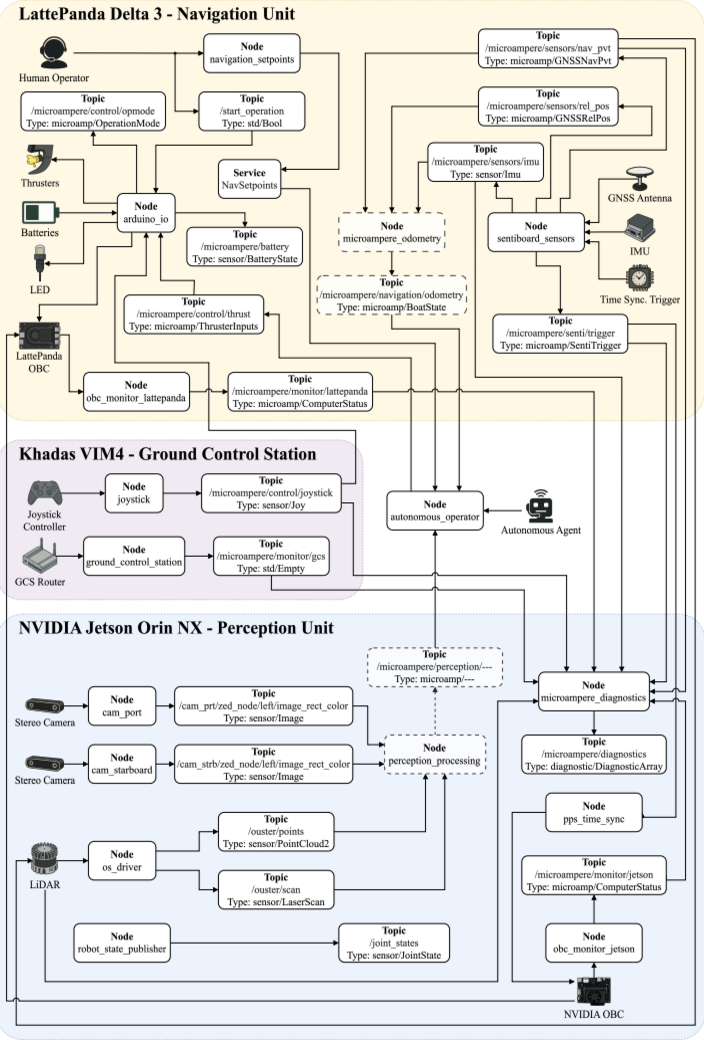
\includegraphics[width=1.0\linewidth]{Pictures/Hardware/Software_Architecture/Overview.png}
    \caption{Overview of the software architecture for the microAmpere ASV, showing the distributed communication between perception, navigation, and control units. Picture taken from Henrik Reimers master thesis on microAmpere ASV.\textsuperscript{\cite{microAmpere_hardware_master_thesis1}}}
    \label{fig:microAmpere-software-architecture-overview}
\end{figure}